%$Header$
% modification history
% Mon Sep 30 13:10:10 CEST 2013 : 
% introduced icmplx, corrected misprint and error on Euler avant in diffusion equation



 \documentclass[triangle]{beamer}
\usepackage{etex}
\DefineNamedColor{named}{lightgray}    {cmyk}{0.0,0,0.0,0.10}
\DefineNamedColor{named}{OliveGreen}    {cmyk}{0.64,0,0.95,0.40}
\DefineNamedColor{named}{DarkGreen}    {cmyk}{0.50,0,0.95,0.40}
\DefineNamedColor{named}{Dandelion}     {cmyk}{0,0.29,0.84,0}
\DeclareMathAlphabet      {\mathup}{OT1}{\familydefault}{m}{n}
\usepackage{algpseudocode}
\def\d{\mathup{d}}
\def\dt{k}
\def\T{^T}
\def\vec{\mathbf}
\def\icmplx{\ensuremath{\dot\imath}}

\newcounter{NumNumericTip}
\newcounter{theexercice}
\newcounter{theexerciceexamen}
\usepackage[]{graphicx}
\usepackage[]{cancel}

 \renewcommand{\CancelColor}{\color{red}}
 \newcommand{\subitem}[1]{\begin{itemize}\item #1\end{itemize}}
 \newcommand{\R}{\texttt{R}}
 \newcommand{\Python}{\texttt{Python}}
\newcommand{\blue}[1]{{\color{blue}#1}}
\renewcommand{\emph}[1]{{\color{purple}#1}}
\usepackage{xcolor}
\usepackage[french]{babel}
\deftranslation[to=french]{Theorem}{Th\'eor\`eme}
\deftranslation[to=french]{Example}{Exemple}
\deftranslation[to=french]{Definition}{D\'efinition}
\usepackage[utf8]{inputenc}
\usepackage{times}
\usepackage[T1]{fontenc}
\usepackage{tikz}
\usetikzlibrary{arrows}
\setbeamertemplate{blocks}[rounded][shadow=true]
\setbeamertemplate{navigation symbols}{}
\setbeamercolor*{block body}{fg=black,bg=yellow!20}
\setbeamercolor*{block body alerted}{fg=black,bg=yellow!30}
\setbeamercolor*{block title}{fg=blue,bg=yellow!30}
\setbeamercolor*{example}{fg=black,bg=blue!30}
\newenvironment{reference}{\begin{block}{Référence}}{\end{block}}


\newenvironment<>{exercice}{%
  \refstepcounter{theexercice}
  \begin{actionenv}#1%
      \def\insertblocktitle{Exercice \arabic{theexercice}}%
      \par%
      \mode<presentation>{%
        \setbeamercolor{block title}{fg=white,bg=orange!20!black}
       \setbeamercolor{block body}{fg=black,bg=olive!50}
     }%
      \usebeamertemplate{block begin}}
    {\par\usebeamertemplate{block end}\end{actionenv}}

\newenvironment<>{exerciceexamen}{%
  \refstepcounter{theexerciceexamen}
  \begin{actionenv}#1%
      \def\insertblocktitle{Exercice d'examen \arabic{theexerciceexamen}}%
      \par%
      \mode<presentation>{%
        \setbeamercolor{block title}{fg=white,bg=orange!20!black}
       \setbeamercolor{block body}{fg=black,bg=red!30}
     }%
      \usebeamertemplate{block begin}}
    {\par\usebeamertemplate{block end}\end{actionenv}}




\newenvironment<>{numerictip}{%
  \begin{actionenv}#1%
     \addtocounter{NumNumericTip}{1}
      \def\insertblocktitle{Astuce numérique  \arabic{NumNumericTip}}%
      \par%
      \mode<presentation>{%
        \setbeamercolor{block title}{fg=white,bg=Dandelion!20!black}
       \setbeamercolor{block body}{fg=black,bg=orange!20}
     }%
      \usebeamertemplate{block begin}}
    {\par\usebeamertemplate{block end}\end{actionenv}}

\setbeamertemplate{footline}{\scriptsize{\hfill\insertframenumber}.\quad\medskip} 
%\usepackage{pgfpages} \pgfpagesuselayout{2 on 1}[a4paper,border shrink=5mm]
\usepackage[all]{xy}	
% \setbeamercolor*{math text inlined}{fg=DarkGreen}

\renewcommand{\d}{\ensuremath{\mathsf{d}}}
\newcommand{\ddt}[1]{\frac{\d#1}{\d t}}
\newcommand{\dddt}[1]{\frac{\d^2#1}{\d t^2}}
\newcommand{\ddd}[2]{\frac{\d^2#1}{\d #2^2}}
\newcommand{\dd}[2]{\frac{\d#1}{\d#2}}
\newcommand{\pdx}[1]{\frac{\partial#1}{\partial x}}
\newcommand{\pdt}[1]{\frac{\partial#1}{\partial t}}
\newcommand{\pd}[2]{\frac{\partial#1}{\partial #2}}
\newcommand{\pdd}[2]{\frac{\partial^2#1}{\partial#2^2}}
\newcommand{\pdxx}[1]{\frac{\partial^2#1}{\partial x^2}}
\newcommand{\pdxt}[1]{\frac{\partial^2#1}{\partial x \partial t}}
\newcommand{\pdtt}[1]{\frac{\partial^2#1}{\partial t^2}}
%\usepackage{natbib}
\bibliographystyle{agu}
\title[Méthodes de Simulation en Physique] % (optional, use only with long paper titles)
{Méthodes de Simulation en Physique}
\setbeamercolor{block text}{fg=black,bg=yellow}
\date

\author%[Author, Another] % (optional, use only with lots of authors)
{ michel.crucifix@uclouvain.be }
\AtBeginSection[]
{
  \begin{frame}<beamer>{Outline}
    \tableofcontents[currentsection,currentsubsection]
  \end{frame}
}

% If you wish to uncover everything in a step-wise fashion, uncomment
% the following command: 

%\beamerdefaultoverlayspecification{<+->}



\begin{document}

\begin{frame}
  \titlepage
\end{frame}

\begin{frame}{Outline}
  \tableofcontents
  % You might wish to add the option [pausesections]
\end{frame}

\section{Introduction}
\begin{frame}
  \frametitle{Ouvrage de référence}
  \begin{columns}
    \column{.3\textwidth} 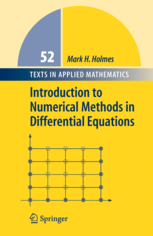
\includegraphics[scale=2]{refbook}
    \column{.7\textwidth} 
     Introduction to Numerical Methods in Differential Equations \\
     Mark H. Holmes \\ Springer Texts in Applied Mathematics (52)

  \end{columns}
\end{frame}
\begin{frame}
  \frametitle{Définition}
  \colorbox{blue!10}{\parbox[l]{\textwidth}
  {\raggedright\Large\bf{
  Résolution algorithmique d'un modèle (physique, chimique, biologique, économique \ldots) analytiquement intractable.
  }
  }
  }
\end{frame}
\begin{frame}{Deux approches complémentaires}
  \begin{enumerate}
    \item Élement d'une démarche théorique
      \begin{itemize}
        \item Étude des propriétés émergentes
        \item Identification d'attracteurs; de points d'(in)stabilité
        \item Mise à l'épreuve de différents modèles
      \end{itemize}
    \item Substitut à un système naturel = outil expérimental
      \begin{itemize}
        \item Expériences d'intervention impossibles à réaliser ou trop coûteuses
        \item Générer des données difficiles à mesurer
        \item Prédiction
      \end{itemize}
  \end{enumerate}
  \begin{block}{Conflit potentiel}
    (1) va vers la simplification / parsimonie. (2) va vers le haut niveau de détail; fidélité au phénomène naturel. 
  \end{block}
\end{frame}


\begin{frame}
  \frametitle{Épistémologie de la simulation}

  \begin{itemize}
    \item Simulateur = dispositif expérimental pour lequel il n'y a pas d'erreur de mesure
    \item Sources d'incertitudes spécifiques, \emph{qu'il faut évaluer}:
      \begin{enumerate}
        \item Choix de représentation physique (modèle)  
        \item Choix d'adaptation au cas particulier
        \item Choix algorithmiques (nombreux et complexes)
        \item Erreurs de codage  
      \end{enumerate}
    \item Role important des outils de visualisation et de post-traitement
      \begin{itemize}
        \item partie intégrante du processus de simulation
      \end{itemize}
  \end{itemize}

  \begin{reference}
    Eric Winsberg, Sanctioning Models: The Epistemology of Simulation,  Science in Context, 12, 275-292  1999  
  \end{reference}
\end{frame}

\begin{frame}
  \frametitle{Contextes de simulation}
  \begin{enumerate}
    \item Résolution d'équations différentielles
      \begin{enumerate}
        \item aux dérivées ordinaires (implique : conditions initiales)
        \item aux dérivées partielles (implique : conditions frontières)
        \item peuvent être stochastiques
      \end{enumerate}
    \item Problèmes d'optimisation (souvent définis comme des problèmes inverses)
    \item Générer des distributions de probabilité
  \end{enumerate}
  \begin{exercice}
    Citer un exemple pour chacun des trois cas de figure
  \end{exercice}
\end{frame}
\begin{frame}
  $\exists$ Deux types de simulateurs: \newline
  Déterministe  $\quad <> \quad $ Stochastique\newline
  \vskip0.5em
  \begin{block}{Simulateurs stochastiques: bien comprendre !}
    Nos ordinateurs sont \textit{toujours} déterministes : \newline
    Les simulateurs stochastiques utilisent des générateurs de pseudo-nombre
    aléatoires\ldots \emph{qu'il faut évaluer} ! \newline
  \end{block}
\end{frame}
\begin{frame}{Approches de programmation}
  \begin{itemize}
    \item Languages compilés : excellente optimisation
      \begin{itemize}
        \item C, C++, Fortran
      \end{itemize}
    \item Languages interprétés : flexibles et conviviaux
      \begin{itemize}
        \item \R, \texttt{python} (\texttt{numpy, scipy})  
        \item Systèmes commerciaux : Matlab, Mathematica \ldots
        \item et clones (octave)
      \end{itemize}
    \item + Librairies standards, optimisées
      \begin{itemize}
        \item  gsl
        \item  LAPACK, BLAS, UMFPACK
        \item \ldots souvent présentes dans les langagues interprétés
      \end{itemize}
  \end{itemize}
  \begin{block}{Mon principe}
    Favoriser les sytèmes open source (communauté internet) permettant des 
    inclusion de code compilé pour les parties critiques. Mes favoris: \R \ et \texttt{numpy / scipy}
  \end{block}
\end{frame}

\section{Problèmes aux conditions initiales}
\begin{frame}
\frametitle{Examples}
\begin{exampleblock}{Décroissance radioactive}
$\ddt{x} = -\lambda x$, \quad avec $x(t_0)=x_0$. \newline
Posons $\hat{x}=x/x_0$ et $\hat{t}=(t-t_0)\lambda$, on a 
\begin{equation}
\dd{\hat{x}}{\hat{t}} = - \hat {x} \quad\text{avec}\quad \hat{x}(0)=1.
\label{eq:rad}
\end{equation}
\end{exampleblock}
\begin{exampleblock}{Equation logistique}
\begin{equation}
\ddt{y}= \lambda y ( 1-y)
\end{equation}
\end{exampleblock}
\begin{exampleblock}{Oscillateur harmonique}
\begin{equation}
\ddt{p}=-\pd{H}{q} \, ; \, \ddt{q}=\pd{H}{p} \quad\text{avec\ } H=\frac{1}{2}(p^2+q^2)
\end{equation}
et $p(0)=p_0$ et $q(0)=q_0$
\end{exampleblock}
\end{frame}
\begin{frame} \frametitle{4 étapes}
De façon générale, le système s'écrit:
\begin{equation}
\ddt{\vec{x}} = \vec{F}(\vec{x}, t)
\end{equation}
\begin{enumerate}
\item Définir les points de discrétisation dans le temps
\item Exprimer le système sous la forme d'une différence finie
\item Laisser tomber l'erreur de troncation
\item Étudier les propriétés : stabilité, convergence, et autres (voir plus loin)
\end{enumerate}
\end{frame}
\begin{frame}\frametitle{1. Discrétisation dans le temps}
\begin{tikzpicture}
 \draw[->](-1, 0) -- ( 7, 0);
 \foreach \i in {0,1,2,3,4,5,6} 
{ \node  at (\i, 0) {$\bullet$};  } 
\foreach \i in {0,1, 2} { \draw (\i, -0.5) node {$t_\i$}; } 
\foreach \i in {6}{ \draw (\i, -0.3) node {$t_n$}; }
\end{tikzpicture}

Dans la suite de ce cours, nous allons poser : 
\begin{itemize}
\item $t_i$ :  le temps discrétisé \\
\item $x(t_i)$ :  la solution exacte au temps $t_i$ \\
\item $x_i$ :  la solution du système en diff. finies au temps $t_i$ \\
\end{itemize}
\begin{example}
\begin{align*}
t_0 &= t(0)  & 
t_i &= t_0 + i\dt
\end{align*}
\end{example}
\end{frame}

\begin{frame}
\frametitle {2. Exprimer le système sous forme de différence finie}
Posons : $F_i := F(x_i, t_i)$. Le problème est d'établir une relation itérative entre $x_i$ et $x_{i+1}$ en utilisant uniquement de l'information disponible aux $t_i$. On 
recourt au développement de Taylor. 
\medskip
On peut faire:
\begin{align}
x(t_{i+1}) &= x(t_i) + F_i k + k\cdot \tau , & \quad \tau &= \dddt {x} (x(t_i),t_i) {k \over 2} + \mathcal{O}(k^2) \label{eq:d1} 
\end{align} ou bien:
\begin{align}
x_(t_{i})   &= x(t_{i+1}) - F_{i+1} k + k\cdot\tau, &\quad \tau &= \dddt {x} (x(t_{i+1}),t_{i+1}) {k\over 2} + \mathcal{O}(k^2) \label{eq:d2}
\end{align}

\end{frame}

\begin{frame}
\frametitle{\ldots et laisser tomber les termes de troncation}

On crée le système aux différences finies en laissant tomber les termes de troncation:

\begin{definition}
Le schéma est dit \textit{consistent} si l'itération converge vers l'expression
du système originel à la limite $k\rightarrow 0$. 
\end{definition}

\begin{center}
\colorbox{yellow!20}
{ \parbox{\textwidth}
{
\begin{tabular}{llll} 
\hline
Euler avant     & (\ref{eq:d1}) & $x_{i+1} = x_i + F_i \dt$ &  $\tau = \mathcal{O}(k)$ \\ 
Euler arrière   & (\ref{eq:d2}) & $x_{i+1} = x_i + F_{i+1} \dt$ & $\tau = \mathcal{O}(k)$ \\ 
Euler centré   & (\eqref{eq:d1} - \eqref{eq:d2}) / 2 &  $x_{i+1} = x_i + F_{i+i/2} k$ & $\tau = \mathcal{O}(k^2)$  \\
\hline
\end{tabular}
où $F_{i+i/2} := {1 \over 2} (F_{i}  + F_{i+1} ) $.
}}
\end{center}

\end{frame}

\begin{frame} \frametitle{Example : décroissance radioactive}

\begin{block}{Euler avant} 
$x_{i+1} = x_{i} - \dt x_{i} = (1-k) x_{i} \Longrightarrow \color{red}{x_i = (1-\dt)^i}x_0$
\end{block}

\begin{block}{Euler arrière} 
$x_{i+1} = x_{i} - \dt x_{i+1}$ : schéma implicite !

$x_{i+1} = (1+\dt)^{-1} x_{i} \Longrightarrow \color{red}{ x_i = (1+\dt)^{-i}}x_0$
\end{block}

\begin{block}{Euler centré} 
$x_{i+1} = x_{i} - {\dt \over 2}(x_{i}+x_{i+1})$ : schéma (semi-implicite)

$x_{i+1} = \frac{1-k/2}{1+k/2} x_{i} \quad \Longrightarrow \quad \color{red}{x_i = \left(\frac{1-k/2}{1+k/2}\right)^i}x_0$
\end{block}
\end{frame}

\begin{frame}
\includegraphics{radio}
\end{frame}

\begin{frame}
\includegraphics{error}
\end{frame}

\begin{frame} \frametitle{Etude des propriétés. I. Convergence}
\begin{block}{Definition} {$\forall t>t_0\, : \, \lim_{k\rightarrow 0} x_i = x(t_i)$} \end{block}
\begin{exampleblock}{Euler avant, radioactivité : (rappel: $x(t_i) = e^{-t}$)}
\begin{align*}
  \log x_{i} &= i \log(1-k) = i ( - k - k^2/2 + \mathcal{O}(k^3) ) = - t - tk/2 + \mathcal{O}(k^3),  \\
 \Rightarrow x_{i} &= e^{-t (1+k/2)} + \mathcal{O}(k^2).
\end{align*}
\end{exampleblock}
\begin{exercice}
Dans cet exemple, l'Euler avant sous-estime la quantité de produit radioactif. Montrer que l'Euler arrière le surestime, et que l'Euler centré est correct au premier ordre.
\end{exercice}
\end{frame}
\begin{frame}
\frametitle{Ordre de grandeur d'approximation du schéma numérique}
\begin{block}{Règle générale}
  Si, étant connu $x_i$, l'approximation sur $x_{i+1}$ est de l'ordre de k$\tau$, alors l'erreur sur la solution à un temps $t$ sera (si $t$ n'est pas trop grand) de l'ordre de $T\cdot\tau$. 
\end{block}
En effet: à chaque pas de temps on accumule une erreur de l'ordre de $k \tau $, et $T/k$ pas de temps sont nécessaires pour intégrer sur une période $T$. 
\end{frame}

\begin{frame} \frametitle{Étude des propriétés. II. stable}
\begin{block}{Définition} Le système est dit \emph{A-stable} si les $x_i$ restent bornés dans le problème de décroissance radioactive. \end{block}
\begin{exampleblock}{Euler avant, radioactivité : }
stable si $|(1-\dt)|\leq1, \quad \Rightarrow \dt\leq2$. 
Le schéma est dit  \emph{conditionnellement A-stable}.
\end{exampleblock}
\begin{exercice}
Déterminer les conditions de stabilité de  l'Euler arrière et l'Euler centré.
\end{exercice}
\end{frame}

\begin{frame} \frametitle{Etude des propriétés. III. monotone}
\begin{block}{Definition} si $x(t_i) < x(t_j)$, alors $x_i < x_j$. \end{block}
\begin{exampleblock}{Euler avant, radioactivité : }
Monotone si $\dt<1$.
Le schéma est dit  \emph{conditionnellement monotone}.
\end{exampleblock}
\begin{exercice}
Déterminer la condition de monotonicité pour l'Euler-centré, et montrer que l'Euler arrière est inconditionnellement monotone. 
\end{exercice}
\end{frame}


\begin{frame} \frametitle{Etude des propriétés. IV. Conserve l'énergie}
S'illustre pour l'oscillateur harmonique. Soit $\vec{x}=(p, q)\T$, 
le problème se formule comme $\ddt {\vec{x}} = M\vec{x}$ où 
$M:=\left( \begin{array}{cc} 0 &-1\\1 &0 \end{array}  \right)$. 

Le problème discrétisé s'écrit
\begin{equation*}
\vec{x}_{i+1} = M_d \vec{x}_i\quad \text{avec}
\end{equation*}
Euler avant : $M_d=(1+M\dt)$; Euler arrière : $M_d=(1-M\dt)^{-1}$ ; 
Euler centré : $M_d=(1-Mk/2)^{-1}(1+M\dt/2)$.

Sachant que le Hamiltonien est ici $\frac{1}{2}x\T x$, l'énergie
augmente de $\vec{x}_i$ à $\vec{x}_{i+1}$ d'un facteur $|{M_d}\T M_d|$.
Ce dernier doit donc être égal à $1$ dans un schéma conservatif. 

\begin{exercice}
Vérifier que le schéma Euler avant crée de l'énergie; que l'Euler arrière en détruit;
et que seul l'Euler centré est conservatif. Illustrer ces propriétés en intégrant le système.
\end{exercice}
\end{frame}

\begin{frame}
\begin{numerictip}
L'opération $M^{-1} x$  (inverse d'une matrice $\times$ vecteur, ou inverse d'une matrice $\times$ matrice) s'effectue efficacement au moyen du package \texttt{LAPACK}, implémenté dans la plupart des langages interprêtés destinés au calcul scientifique:
\medskip
\begin{tabular}{ll}
\hline
matlab / octave : & \texttt{M  $\setminus$ x} \\
R  : & \texttt{ solve(M, x) } \\
numpy / scipy : & \texttt{ np.solve(M, x) }  \\
\hline
\end{tabular}
\end{numerictip}
\end{frame}


\begin{frame}
\includegraphics{oscillateur_euler}
\end{frame}

\begin{frame}
\frametitle{Schéma leap-frog}
\begin{block}{Idée}
Mimer le schéma centré, mais selon un schéma explicite à deux pas de temps
\begin{equation}
x_{i+1} = x_{i-1} + 2\dt F(x_i)
\end{equation}
\end{block}

nécessite d'initialiser $x_0$ et $x_1$.

\begin{exercice}
Démontrer que le schéma leap-frog est instable dans le problème de décroissance radioactive. 
Indice : tenter une solution $x_i = \alpha^i$ et chercher les solutions pour $\alpha$. 
Le schéma est instable si $|\alpha|>1$. 
\end{exercice}
\end{frame}

\begin{frame}
\includegraphics{radio_leapfrog}
\end{frame}

\begin{frame}
\frametitle{Schéma de Heun (RK2)}
\begin{block}{Idée}
Approximer $F_{i+1}$ par $\tilde{F}_{i+1} := F(x_i + k F(x_i), t_{i+1})$. Peut se réecrire comme:
\begin{align*}
\tilde{x}_{i+1} &= x_i + \dt F_i \\
x_{i+1} &= x_i + {k \over 2}\left(F\left(x_i, t_i \right) + F\left(\tilde{x}_{i+1}, t_{i+1}\right)\right),
\end{align*}
qui fait apparaître la notion \emph{prédicteur - correcteur}.
\end{block}
%
\begin{exercice}
Développer $\tilde{F}_{i+1}$ en série autour de $F(x_i)$ et montrer que la méthode de Heun est
convergente à l'ordre 2 en k.
\end{exercice}
\end{frame}
\begin{frame}
\frametitle{Schéma de Runge-Kutta d'ordre 4 (RK4)}
\begin{align*}
k_1 &= k\cdot F_i \\
k_2 &= k\cdot F(x_i + k_1/2, t_i + k/2) \\
k_3 &= k\cdot F(x_i + k_2/2, t_i + k/2) \\
k_4 &= k\cdot F(x_i + k_3, t_i + k) \\
x_{i+1} &= x_i + {1\over 6}\left( k_1 + 2 k_2 + 2 k_3 + k_4 \right)
\end{align*}
\begin{block}{propriétés}
\begin{itemize}
\item Explicite
\item Conditionnellement stable
\item Troncation d'ordre 5; solution convergente à l'ordre 4.
\end{itemize}
\end{block}
\end{frame}
%

\begin{frame}
\includegraphics{error_withRK4}
\end{frame}

\begin{frame}
\begin{exercice}
L'équation logistique :
\begin{equation}
\ddt {x} = \lambda x ( 1-x)\, \quad x{0}=\alpha 
\end{equation}
a pour solution exacte:
\begin{equation}
x(t) = \frac{\alpha}{\alpha +   (1 - \alpha ) e^{-\lambda t }}.
\end{equation}
Comparer les erreurs des schémas explicites Euler avant, Heun et RK4 pour différents pas de temps comme sur la figure précédente. 
\end{exercice}

\begin{exercice}
Le schéma Euler arrière peut s'établir analytiquement pour l'équation logistique, mais cela implique de résoudre, à chaque pas de temps, une équation du second degré,\ldots qui a donc deux solutions. Laquelle des deux solutions retenir?
\end{exercice}
\end{frame}

\begin{frame}
\frametitle{Erreurs d'arrondi (erreur machine)}
\begin{numerictip}  
Dans l'opération $a+b$, $|log_2(a)-log_2(b)|$  doit être plus grand que $m$, où
$m$ est le nombre de bits réservés pour la mantisse:
\begin{center}
\begin{tabular}{l|l|l}
type & m & $ log_{10} (2^m)$\\
\hline
float16 & 10 &  $3.0 $\\
float32 & 23 & $6.9 $\\
float64 & 52 & $15.6$\\
float128& 64 & $19.2$\\
float256 & 112 & $33.7$ \\
\hline
\end{tabular}
\end{center}
\end{numerictip}
\end{frame}

\begin{frame}
\includegraphics{rounding_error}
\end{frame}


\begin{frame} \frametitle{Schémas symplectiques}
Reprenons l'oscillateur harmonique, et considérons :
\begin{exampleblock}{Le schéma Verlet}
\begin{align*}
\tilde{p}_{i+1} &= p_i - \dt  q_i \\
q_{i+1} &= q_i + {\dt\over 2} (p_i + \tilde{p}_{i+1} ) \\
p_{i+1} &= p_i - {\dt\over 2} (q_i + q_{i+1} ) 
\end{align*}
\end{exampleblock}
\end{frame}

\begin{frame}
\includegraphics{oscillateur_energy1}
\end{frame}

\begin{frame}
\includegraphics{oscillateur_energy2}
\end{frame}

\begin{frame}
\frametitle{Méthode symplectique = respecte la géométrie du problème}
\begin{columns}
\column{0.45\textwidth}
\begin{tikzpicture}
 \draw [-open triangle 60] (-0.5, 0) -- (3, 0) node [below] {$q$}; 
 \draw [-open triangle 60] ( 0, -0.5) -- (0, 3) node [left] {$p$}; 

 \draw [-open triangle 60] ( 0.5, 0.7) node [below] {$x^a_{i}$} -- (1.3, 2.7) node [left] {$x^b_{i}$}; 
 \draw [-open triangle 60] ( 0.5, 0.7) -- (2.5, 0.9) node [right] {$x^c_{i}$}; 
 \draw [dashed] ( 2.5, 0.9) -- (3.3, 2.9) -- (1.3, 2.7) ; 
\end{tikzpicture}

\column{0.45\textwidth}
\begin{tikzpicture}
 \draw [-open triangle 60] (-0.5, 0) -- (3, 0) node [below] {$q$}; 
 \draw [-open triangle 60] ( 0, -0.5) -- (0, 3) node [left] {$p$}; 

 \draw [-open triangle 60] ( 0.5, 0.7) node [below] {$x^{a}_{i+1}$} -- (1.3, 2.2) node [left] {$x^{b}_{i+1}$}; 
 \draw [-open triangle 60] ( 0.5, 0.7) -- (3.0, 0.9) node [right] {$x^{c}_{i+1}$}; 
 \draw [dashed] ( 3.0, 0.9) -- (3.8, 2.4) -- (1.3, 2.2) ; 
\end{tikzpicture}
\end{columns}
Le schéma symplectique conserve l'aire des parallélogrammes (dans une métrique donnée)
\begin{theorem}
Soit $p_{i+1}=f(p_i, q_i)$ et $q_{i+1}=g(p_i, q_i)$. Alors le schéma est symplectique ssi
$\left| \begin{array}{cc}f_p & f_q \\ g_p & g_q \end{array}\right|=1, \ \forall{p, q}.$
\end{theorem}
\end{frame}
\begin{frame}
\begin{exercice}
Montrer que la méthode de Heun n'est pas symplectique pour l'oscillateur Harmonique; mais que la méthode de Verlet l'est bien.
\end{exercice}
\end{frame}

\section{Problèmes aux conditions frontières}
\begin{frame}
\begin{exampleblock}{Tension sur un fil}
\begin{equation} \ddd{y}{x} = f(x), \text{pour} \quad  0<x<\ell \quad \text{avec}\, y(0)=y(\ell)=0.  \end{equation}
\end{exampleblock}

\begin{exampleblock}{Équation de Bratu (cinématique chimique)}
\begin{equation} \ddd{y}{x} = - e^y, \text{pour} \quad 0<x<\ell \quad \text{avec}\, y(0)=y(\ell)=0.  \end{equation}
\end{exampleblock}

\end{frame}
\begin{frame} \frametitle{Méthode des différences finies}
\begin{enumerate}
\item Définir les points de discrétisation $x_0, x_1, \ldots, x_{N+1}$.
\item Évaluer l'équation différentielle en ces points
\item Exprimer la dérivée sous la forme d'une différence finie
\item Laisser tomber les termes de troncature.
\end{enumerate}
\end{frame}

\begin{frame}
\frametitle{Corde sous tension : résolution par différence finie}
\begin{enumerate}
\item On choisit:  $$x_i = ih, \quad i=0,1, \ldots , N+1.$$
\item On a donc: $$\ddd{y}{x}(x_i) = f(x_i) =: f_i$$
\item On exprime : $$\ddd{y}{x}(x_i) = \frac{y_{i+1} - 2y_i + y_{i-1}}{h^2} + \mathcal{O}(h^3),$$
\item Ce qui donne : $$y_{i+1} - 2y_i + y_{i-1}  = h^2 f_i.$$
\end{enumerate}
\end{frame}

\begin{frame}
Le système s'écrit donc dans ce cas comme une équation linéaire, à matrice tri-diagonale:
\begin{equation}
\left( 
\begin{array}{rrrrr}
 -2 &  1 &    &     \\
  1 & -2 &  1 &     \\
    &\ddots& \ddots   & \ddots    \\
    &  1 &-2  &  1 \\
    &    & 1  & -2 \\
\end{array}
\right)
\left( 
\begin{array}{c}
 y_1 \\ y_2  \\  \vdots  \\ y_{N-1} \\ y_{N}
\end{array}
\right) = 
h^2
\left(
\begin{array}{c}
f_1 \\  f_2  \\   \vdots  \\ f_{N-1} \\  f_{N} 
\end{array}
\right )
\end{equation}
\end{frame}
\begin{frame}\frametitle{Matrices tri-diagonales}
\begin{numerictip}
\begin{tabular}{cc}
\parbox{0.45\textwidth} 
{
Les équations à matrices tri-diagonales, de la forme $\vec{Ay}=\vec{z}$, où
$\vec{A}=
\left( 
\begin{array}{lllll}
 a_1& c_1 &    &     \\
 b_2 & a_2 & c_2 &     \\
    &\ddots& \ddots   & \ddots    \\
    & b_{N-1} & a_{N-1}  &  c_{N-1} \\
    &    &b_N &  a_{N} \\
\end{array}
\right)$, se résolvent selon un algorithme simple, dérivé de la factorisation LU:
}
& 
\colorbox{yellow!10}{\parbox{0.45\textwidth}{
\begin{algorithmic}[1]
\State $w \gets  a_1$; $y_1 \gets z_1 / w $
\For {$i=2 \to N$}
\State $v_i \gets {c_{i-1} / w}$
\State $w \gets a_i - b_i v_i$
\State $y_i \gets {(z_i - b_i y_{i-1}) / {w}}$
\EndFor
\For {$j=N-1, N-2, \ldots , 1$}
\State $y_i \gets y_i - v_{j+1} y_{j+1}$
\EndFor
\end{algorithmic}
}
}
\end{tabular}
\bigskip

Bien sûr, \texttt{LAPACK} fait ceci pour vous.
\end{numerictip}
\end{frame}

\begin{frame}
\frametitle{Solution unique du système en diff. finie?}
Soit les sommes partielles $r_i$, définies comme la somme des éléments non-diagonaux sur la ligne $i$, i. e. 
$$ 
r_i = \left\{ \begin{array}{ll} 
   |b_i| + |c_i| \quad & \text{si} i \neq 1,N, \\
   |c_1|  & \text{si} i = 1, \\
   |b_N|  & \text{si} i = N, \end{array}\right.
$$
\begin{definition} 
Une matrice est dite tridiagonalement dominante si $|a_i| \geq r_i\, \forall i$, et strictement dominante si l'inégalité est stricte.
\end{definition}
\begin{theorem}
Une matrice admet une inverse réelle soit si, 
\begin{enumerate}
\item elle est strictement diagonalement dominante
\item elle est diagonalement dominante, avec $c_i\neq 0\, \forall i$, et $|b_N|<|a_N|$.
\end{enumerate}
\end{theorem}
\end{frame}
\begin{frame}
\frametitle{Solution unique? (suite)}
On voit donc que pour le probl\`eme de la corde sous tension, la solution sera toujours unique, quelle que soit la r\'esolution spatiale. 

L'\'equation plus g\'en\'erale:
\begin{equation}
\ddd{y}{x} + p(x) \dd{y}{x} + q(x)y = f(x)
\label{eq:gen}
\end{equation}
admet pour résolution en différence finie:
\begin{eqnarray*}
&a_i = - 2 + h^2q(x_i) ; \quad b_i=1-\frac{h}{2}p(x_i);\quad c_i=1+\frac{h}{2}p(x_i)
\end{eqnarray*}
On peut montrer (Holmes, p. 52) que  \label{solunique}
\begin{theorem}
si $p(x)$, $q(x)$ et $f(x)$ sont continues, et que $q(x)\leq0$, alors la solution est unique si $hp_\infty < 2$, o\`u $p_\infty :=\max |p(x)|$.
\end{theorem}
\end{frame}
\begin{frame}\frametitle{Matrice bien conditionnée?}
\begin{definition}
 La condition Euclidienne d'une matrice, noté $\mathop{cond}_2$ est le rapport en valeur absolue entre sa plus petite et sa plus grande valeur propre. 
\end{definition}

\begin{numerictip}
 La résolution numérique de l'inverse d'une matrice n'est fiable que si l'inverse de sa condition est grand par rapport à l'erreur de troncature. 
\end{numerictip}
\end{frame}

\begin{frame}
La matrice
$\vec{A}=
\left( 
\begin{array}{ccccc}
 a& c &    &     \\
 b & a & c &     \\
    &\ddots& \ddots &    \\
    & b & a  &  c \\
    &    &b &  a \\
\end{array}
\right)$, admet pour valeurs propres (cf. \url{http://files.itslearning.com/data/ntnu/open/CO33563/1433595.pdf})

\begin{equation}
\lambda_i = a + 2 \sqrt{bc} \cos \left( \frac{i\pi}{N+1} \right).
\end{equation}

On peut vérifier que pour le problème général \eqref{eq:gen} mais avec $p(x)\equiv p$, $q(x)\equiv q$, et en développant les termes en $\cos$ selon Taylor, que
\begin{equation*}
\mathop{cond}_2(\vec{A}) = \frac{16N^2}{4\pi^2 + \left( p^2 - 4q \right)\ell^2} + \mathcal{O}(N).
\end{equation*}
\end{frame}

\begin{frame}
\begin{example}
\includegraphics{bvp_prob1}
\end{example}
\end{frame}

\begin{frame}
\frametitle{Analyse d'erreur}
L'erreur totale peut se décomposer en $|(y(x_i) - y_i) + (y_i - \bar{y}_i)|$, où
\begin{tabular}{ll}
\quad & $y_i$ est la solution du système en différence finie \\
\quad & $\bar{y}_i$ est la solution calculée par ordinateur (numérique)
\end{tabular}

\begin{theorem}
Si les fonction $p$, $q$, $f$ sont continues, et $q(x) \leq -\gamma < 0$, alors
\begin{equation*}
|(y(x_i) - y_i)| \leq C \left[\tau_\infty + \mathop{max}\left\{ |E_0||E_{N+1}| \right\} \right],
\end{equation*}
où $\tau_\infty$ est la plus grande erreur de troncature du schéma, $C=\mathop{max}\left\{ 1,1/\gamma \right\}$, et $E_0$ et $E_\infty$ sont les approximations éventuelles des conditions frontières.
\end{theorem}

Le terme $|(y_i - \bar{y}_i)| $ devient potentiellement important lorsque la matrice est mal conditionnée. 

\end{frame}

\begin{frame}
\begin{example}
\includegraphics{bvp_error.pdf}
\end{example}
\end{frame}

\begin{frame}
\begin{exercice}
Le système suivant illustre la notion de couche limite: 
\begin{equation}
\epsilon \ddd{y}{x} - x^2 \dd{y}{x} - y = 0, \quad 0 < x < 1, \epsilon=10^{-2},
\end{equation}
avec les conditions frontières : $y(0)=y(1)=1$. 
Calculez en les solutions en différence finie pour $N=10, 20, 50, 120$. 
Comparez avec le critère garantissant la solution unique (p. \pageref{solunique}).
Qu'en déduisez-vous? A partir de quelle valeur de $N$ peut-on penser que les erreurs d'arrondi 
vont commencer à dominer? Sur base de ces considérations, quel intérêt tirerait-on d'une grille non régulière dans un cas comme celui-ci?
\end{exercice}
\end{frame}
\begin{frame}
\includegraphics{bvp_prob2.pdf}
\end{frame}

\begin{frame}
\frametitle{Conditions sur les dérivées}
Les conditions frontières peuvent s'imposer sur les dérivées $\dd{y}{x}(0, \ell)$, où même une combinaison des dérivées et des valeurs aux frontières.
\begin{example}
La condition $a\, y(0) + b \, \dd{y}{x}(0) = \alpha$ peut elle même s'exprimer sous la forme d'une différence finie. Pour bien faire, il nous faut une approximation d'ordre 2. L'approximation suivante en est une:
\begin{equation*}
a\, y_0 + \frac{b}{2h}(-y_2 + 4 y_1 - 3 y_0) = \alpha
\end{equation*}
qui peut se réexprimer sous la forme:
\begin{equation*}
y_0 = \frac{b}{2ah - 3b}(y_2 - 4 y_1) + \frac{2 \alpha h}{2 a h - 3b}
\end{equation*}

On peut alors utiliser cette valeur de $y_0$ lorsqu'on développe la matrice $\vec{A}$.
\end{example}
\end{frame}

\begin{frame}
  \begin{exercice}
    Considérons le problème général
    \begin{equation*}
      y^{\prime\prime} + p(x) y^\prime + q(x) y = f(x)\, \text{pour }0<x<\ell
    \end{equation*}
    Développez de schémas en diff. finies corrects à l'ordre 2 pour les conditions
    (deux exercices distincts)
    \begin{enumerate}
      \item $y(0)=\alpha \quad\text{et}\quad y(\ell)+\gamma y^\prime(\ell) = \beta $ \\
      \item $y(0)=y(\ell)$ \quad\text{et}\quad $y^\prime(0)=y^\prime(\ell)$ 
    \end{enumerate}
  \end{exercice}
\end{frame}


\begin{frame}
\frametitle{Systèmes non linéaires}
De façon tout à fait générale, l'approximation en différence finie d'un système non-linéaire va pouvoir s'exprimer sous la forme
\begin{equation}
\vec{F}(\vec{y}) = \vec{0}
\label{}
\end{equation}

Que l'on peut résoudre selon la méthode de Newton. Soit:  \\
\begin{tabular}{ll}
\quad & $\vec{z_0}$ une estimation de ce que la solution peut être \\
\quad & $\vec{J}$ le Jacobien de $F$.
\end{tabular}

Le schéma suivant doit converger vers la solution si le système est suffisamment régulier:
\begin{equation*}
\vec{z}_{k+1} = \vec{z}_k - {J_k}^{-1} \vec{F_k}, \quad k=0, 1, 2, \ldots
\end{equation*}
\begin{exercice}
Résoudre l'équation de Bratu $y^{\prime \prime}=-e^{y}$, $0<x<1$, avec $y(0)=y(1)=0$. 
Utiliser comme premier essai $z_0=x-x^2$; recommencez et utilisez $z_0=16 (x-x^2)$. Qu'en déduisez-vous?
\end{exercice}
\end{frame}
\begin{frame}
\includegraphics{bratu}
\end{frame}
\begin{frame}
\frametitle{Autres méthodes}
\begin{block}{Méthodes des résidus}  Exprimer $y(x)$ dans un base de fonctions ($y(x)=\sum a_i \phi_i(x)$) et ajuster les coefficients (collocation ou moindre carrés : voir cours Prof. B. Piraux)
\end{block}
\begin{block}{Shooting methods}
Reformuler le problème de façon similaire à un problème aux conditions initiales, i.e. : $\dd{x}{\vec{y}}=F(x, {y})$ où $\vec{y}=(y, y^\prime)\T$ et où seul $\vec{y}(0)$ est spécifié, et ajuster itérativement la condition sur $\vec{y}(0)$ de façon à remplir  les conditions frontières en $x=0$ et $x=\ell$.
\end{block}
\end{frame}
\section{Equation de diffusion}
\begin{frame}
\frametitle{Définition}
La forme générale de l'\'equation de diffusion s'écrit:
\begin{equation}
a(x, t) \pdxx{u} + b(x, t) \pdx{u} + c(x, t) u = \pdt u + f(x, t), \quad
\text{pour } \left\{ \begin{array}{l} 0 < x < \ell, \\ 0 < t. \end{array} \right..
\label{eq:chaleur}
\end{equation}
Nécessite des conditions initiales \emph{et} des conditions aux frontières. 
\end{frame}
\begin{frame}
\begin{example}
L'équation de la chaleur (adimensionnelle) se réduit à $a(x, t) = 1$; $b=c=f=0$. \\
Si on admet, pour conditions ($\ell = 1$):
$$u(0, t)= u(1, t)=0 \quad \text{ pour }\ t>0\text{, et} $$
$$u(x, 0) = g(x), \quad \text{pour } 0 \leq x \leq 1, $$
alors le système admet pour solution \footnote{truc: écrire $u=A(x)C(t)$}:
\begin{equation}
u(x, t) = \sum_{n=1}^{\infty} A_n e^{-\lambda_n^2 t} \sin (\lambda x),
\label{}
\end{equation}
où $\lambda_n=n\pi$ et $A_n = 2 \int_0^{1} g(x) \sin (\lambda x)\, \d x$
\end{example}
\end{frame}
\begin{frame}
\begin{exercice}
\label{eqchal}
Déterminer les solutions analytiques de l'équation de la chaleur adimensionnelle définie page prédente, pour
\begin{enumerate}
\item $g(x) = \sin(2\pi x)$, 
\item $g(x) = \left\{ \begin{array}{ll} 1\quad & \text{si \ } a \leq x \leq b, \\ 0 & sinon. \end{array} \right.$
\end{enumerate}
\end{exercice}
\begin{block}{Propriétés de l'équation de la chaleur}
\begin{itemize}
\item La solution est continuement dérivable à l'intérieur des frontières
\item Les minima et maxima se trouvent aux frontières, soit latérales, soit en $t=0$.
\item L'information se propage instantanément (illustration: cas 2. de l'exercice ci-dessus)
\end{itemize}
\end{block}
\end{frame}
\begin{frame}
\frametitle{Résolution en 4 étapes}
\begin{enumerate}
\item Définir les points de discrétisation
\item Estimer le système en ces points
\item Le formuler en différences finies
\item Éliminer les termes de troncature
\end{enumerate}
\end{frame}
\begin{frame}
\frametitle{1. Discrétisation}
\begin{tikzpicture}[xscale=1.3]
\draw [->] (-0.2, 0) -- (4.8, 0) node [yshift=-1em] {$x$} ; 
\draw [->] (0, -0.2) -- (0, 4.8) node [xshift=-1.5em] {$t$} ;
\foreach \i in {1, 2, 3}
 { 
 \draw (\i, 0) node [yshift=-1em] {$x_\i$} -- (\i, 4) ; 
 \draw (0, \i) node [xshift=-1.5em] {$t_\i$} -- (4, \i) ; 
 \foreach \j in {1, 2, 3, 4}
  { \node at (\i, \j)  [shape=circle, draw, color=black] {} ; }
  }
  \draw ( 4, 0) node [yshift=-1em] {$\ell$} -- ( 4, 4) ; 
  \draw ( 0, 4) node [xshift= -1.5em] {$t_4$} -- ( 4, 4) ; 

  \foreach \j in {0,1, 2, 3,4}
  { \node at (\j, 0 )  [shape=circle, draw, color=black, fill=black!30] {} ; 
    \node at (0 , \j)  [shape=circle, draw, color=black, fill=black!30] {} ; 
    \node at (4 , \j)  [shape=circle, draw, color=black, fill=black!30] {} ; }

\end{tikzpicture}

Pour un grille régulière, on aura $t_j = j \dt$ et $x_i = i h $. 
\end{frame}

\begin{frame}
\frametitle{2. : exprimer le système aux points de grille}
Nous reprenons l'équation de la chaleur, cette fois non-homogène :
\begin{equation*}
\pdxx{u} = \pdt{u} + f(x, t),
\end{equation*}
avec $u(0, t) = u(1, t) = 0$; $u(x, 0) = g(x)$, et nous adoptons pour notation: \\
$u_t := \pdt{u}$, $u_x := \pdx{u}$, $u_{xx} := \pdxx{u}$ etc. 

\bigskip

Le système discrétisé est donc : 
\begin{equation}
u_{xx} (x_i, t_j) = u_t (x_i, t_j) + f (x_i, t_j)
\label{}
\end{equation}

\end{frame}
\begin{frame}
\frametitle{3. Exprimer le système sous forme de différence finie}
On choisit un schéma centré dans l'espace:
\begin{align*}
u_{xx}(x_i, t_j) &= \frac{u(x_{i+1}, t_j) - 2u (x_i, t_j) + u(x_{i-1}, t_j)}{h^2} + \mathcal{O}(h^2)
\end{align*}
et Euler avant dans le temps:
\begin{align*}
u_t(x_i, t_{j}) &= \frac{u(x_i, t_{j+1}) - u (x_i, t_{j})}{k} + \mathcal{O}(k)
\end{align*}
\end{frame}
\begin{frame}
\frametitle{4. \ldots et on laisse tomber les termes de troncature.}
Posons $\lambda = k / h^2$, on a:
\begin{equation}
u_{i, j+1} = \lambda u_{i+1, j} + (1-2\lambda) u_{i,j} + \lambda u_{i-1, j} - k f_{i,j},
\label{}
\end{equation}
ce qui peut s'écrire sous la forme 
\begin{align*}
\vec{u}_0 &= \vec{g}  \\
\vec{u}_{j+1} &=  (1-\vec{H})\vec{u}_{j} - k \vec{f}_j, \quad \text{pour\ }j = 1\ldots M-1\\
\end{align*}
\begin{columns}
\column{0.35\textwidth}
où : 
\begin{align*}
 \vec{u}_j &= (u_{1, j}, u_{2, j}, \ldots , u_{N, j} ) \\
 \vec{f}_j &= (f_{1, j}, f_{2, j}, \ldots , f_{N, j} )  \\
 \vec{g} &= (g_{1}, g_{2}, \ldots , g_{N} )  \\
\end{align*}
\column{0.55\textwidth}
et $\vec{H}=\left( 
\begin{array}[h]{cccc}
  2\lambda &  -\lambda  &          &           \\

-\lambda    &  2\lambda & -\lambda  &           \\

           &\ddots     & \ddots    & \ddots    \\

           &           &-\lambda    &  2\lambda   \\

\end{array}
\right)$
\end{columns}
\end{frame}
\def\stencil{
 \draw [-] (-1.8, 0) node [left] {$t_j$} -- (1.8, 0); 
 \draw [-] (-1.8, 1) node [left] {$t_{j+1}$} -- (1.8, 1); 
 \draw [-] (-1, -0.5) node [yshift=-1.5em] {$x_{i-1}$} -- (-1, 1.5 ); 
 \draw [-] (0, -0.5) node [yshift=-1.5em] {$x_{i}$} -- (0, 1.5 ); 
 \draw [-] (1, -0.5) node [yshift=-1.5em] {$x_{i+1}$} -- (1, 1.5 ); 
 \node at (0,1)  [shape=circle, draw, color=black] { } ; 
 }


\begin{frame}
Le \emph{stencil} représente les points dont dépend le calcul du $u_{j+1, i}$:
\begin{tikzpicture} 
 \stencil
 \foreach \i in {-1, 0, 1} {\node at (\i,0)  [shape=circle, draw, fill=black!30] { } ; } 
\end{tikzpicture}

Le système qui nous occupe est donc \emph{explicite.}
Ce schéma Euler avant de l'équation de la chaleur admet une solution analytique  si $\vec{f}=0$:

\framebox[\textwidth]
{
si $\vec{u}_0=w_0 e^{rx\dot\imath}$, alors
$\vec{u}_n=(1-q)^n \vec{u}_0$, où $q=4\lambda \sin^2\left( \frac{rh}{2} \right)$.
}

($\icmplx:= \sqrt{-1}$)
\end{frame}

\begin{frame}

\renewcommand\arraystretch{2.4} 
\begin{tabular}{l|l|l}
%\setlength\minrowclearance{2.4pt}
\textbf{schéma} & \textbf{Itération} & \textbf{Solution analytique$^\star$ }\\
\hline
E. avant & $\vec{u}_{j+1} =  (1-\vec{H})\vec{u}_{j}  $ & $\vec{u}_n=(1-q)^n \vec{u}_0$  \\
\hline
E. arrière & $(1+\vec{H})\vec{u}_{j+1} =  \vec{u}_{j} $ & $\vec{u}_n=(1+q)^{-n} \vec{u}_0 $  \\
\hline
CN & $(1+\vec{H}/2)\vec{u}_{j+1} =  (1-\vec{H}/2)\vec{u}_{j} $ & $\vec{u}_n=\left(\frac{1-q/2}{1+q/2}\right)^n \vec{u}_0$  \\
\end{tabular}
\renewcommand\arraystretch{1.2} 
\bigskip
\begin{tabular}{ll}
E. avant : & Euler avant \\
E. arrière : & Euler arrière \\
CN : & Crank - Nicholson 
\end{tabular}

$\star: $ solution pour $\vec{u}_0 = w_0 e^{rx\icmplx}$ 

\begin{exercice}
Lesquelles de ces méthodes préservent la propriété de propagation instantanée ?
\end{exercice}
\end{frame}

\begin{frame}
\frametitle{Stabilités A et L}
Définissons $k(q)$ tel que $\vec{u}_{i+1} = k \vec{u}_{i} $, $\vec{u}_{0}=w_0 e^{\icmplx rx}$:
\begin{definition}
Une méthode est dite \emph{L-stable} si $\lim_{q\rightarrow \infty} k(q) = 0$
\end{definition}
\begin{exercice}
Discutez les stabilités A (i.e.: solution bornée) et L des trois méthodes ci-dessus. Illustrez votre réponse en codant l'équation de la chaleur et en la résolvant et montrant la solution à $t=0.1$, $N=12$, $\lambda=0.5, 1.5, 2.5$ et pour la fonction $g$ telle que définie dans l'exercice \ref{eqchal} cas 2, avec $a=\frac{1}{4}$ et $b=\frac{3}{4}$. 
\end{exercice}
\end{frame}

\begin{frame}
\includegraphics{heat_0.pdf}
\end{frame}

\begin{frame}
\includegraphics{heat_1.pdf}
\end{frame}

\begin{frame}
\includegraphics{heat_xl_1.pdf}
\end{frame}


\begin{frame}
\includegraphics{heat_xl_2.pdf}
\end{frame}

\begin{frame}
\includegraphics{heat_3d.pdf}
\end{frame}
\section{Équation d'advection}
\begin{frame}
De façon générale l'équation d'advection s'écrit
\begin{equation}
\pdt{u} + a \pdx {u} = 0,\quad \text{pour}\ \left\{ \begin{array}{ll} -\infty < x < \infty, \\ 0 < t, \end{array} \right.
\end{equation}
avec la condition frontière $u(x,0)=g(x)$.
\end{frame}
\begin{frame}
\frametitle{Résolution analytique}
Définissons $(r,s)$ tels que : $x = ar+s$ et $t = r$. Alors:
\begin{equation}
\pdd{u }{r} = \pdd{u}{t} \pdd{t}{r} + \pdd{u}{x} \pdd{x}{r} =  \pdt{u} + a \pdx {u} = 0.
\label{}
\end{equation}
\begin{tabular}{ll}
Donc: $u(x(r,s), t(r,s))$&$=u(ar+s, r)$ est invariant $\forall r=t$, \\ & $= u(s, 0) = g(x-at)$.
\end{tabular}
\end{frame}
\newcommand{\setcol}[1] { 
 \ifnum#1=0 %
 \def\fcol{red} \fi
 \ifnum #1=1 \def\fcol{blue} \fi
 \ifnum #1=2 \def\fcol{black} \fi
 }

\begin{frame}
\begin{example}
$a=1$ et $g(x)=e^{-x^2}$

\bigskip

\begin{tikzpicture}
\draw [->] (-5,0) -- (3,0) node [below] {$x$};
\foreach \i in {0,1,2}
{ \setcol{\i} \draw [color=\fcol] plot[id=f\i,domain=-5+\i:-1+\i] function {exp(-(x+3-\i)*(x+3-\i))} node [xshift=-4em, yshift=4em] {$t=\i$}; }
\foreach \i in {-1,...,5} { \draw (\i-3, 0) -- (\i-3, -0.1) node [below] {\small{$\i$}}; } 
\end{tikzpicture} 
\end{example}
\begin{block}{propriétés}
\begin{itemize}
\item Information se propage sans déformation à vitesse $a$
\item La solution en $(x,t)$ est entièrement déterminée par l'information en $\bar{x}=x-at$.
\end{itemize}
\end{block}
\end{frame} 

\begin{frame}
\begin{tikzpicture}
\draw [->] (-1,0) -- (4,0) node [below] {$x$};
\draw [->] (0,-1) -- (0,3.2) node [left] {$t$};
\node at (4,2) {$\bullet$};
\draw [color=black!50] (1,0) node [below] {$(x-at,0)$} -- (2.5, 1) node [right] {$\longleftarrow$ \parbox{4em}{\small {domaine de dépendence}}} -- (4,2) node [right] {$(x,t)$};
\end{tikzpicture}
\end{frame}

\begin{frame}
\frametitle{Schéma upwind}
On part de l'équation en différence finie:
\begin{align*}
\frac{u(x_i, t_{j+1}) - u(x_i, t_{j}) }{k} + a \frac{u(x_i, t_{j}) - u(x_{i-1}, t_{j}) }{h} + \tau_{ij} &= 0,  \\
\tau_{ij} &= \mathcal{O}(h) +  \mathcal{O}(k).
\end{align*}
\end{frame}
\begin{frame}
\frametitle{Schéma downwind}
On part de l'équation en différence finie:
\begin{align*}
\frac{u(x_i, t_{j+1}) - u(x_i, t_{j}) }{k} + a \frac{u(x_{i+1}, t_{j}) - u(x_{i}, t_{j}) }{h} + \tau_{ij} &= 0,  \\
\tau_{ij} &= \mathcal{O}(h) +  \mathcal{O}(k).
\end{align*}
\end{frame}

\begin{frame}
\begin{tabular}{l|l}
upwind  & downwind \\ \hline \\
\begin{tikzpicture}
\stencil
 \node at ( -1 , 0)  [shape=circle, draw, fill=black!30] { } ; 
 \node at ( 0,0)  [shape=circle, draw, fill=black!30] { } ; 
 \node at ( 0,1)  [shape=circle, draw] { } ; 
\end{tikzpicture}  
&
\begin{tikzpicture}
\stencil
 \node at (1 ,0)  [shape=circle, draw, fill=black!30] { } ; 
 \node at ( 0,0)  [shape=circle, draw, fill=black!30] { } ; 
 \node at ( 0,1)  [shape=circle, draw] { } ; 
\end{tikzpicture} 
\\
\parbox{0.4\textwidth}{
\begin{align*}
u_{i,j+1} &= (1-\lambda) u_{ij} + \lambda u_{i-1,j}, \\
\lambda   &= ak / h
\end{align*}
}
& 
\parbox{0.4\textwidth}{
\begin{align*}
u_{i,j+1} &= (1+\lambda) u_{i,j} - \lambda u_{i+1,j}, \\
\lambda   &= ak / h
\end{align*} 
}
\\
\hline
\end{tabular}
\end{frame}

\newcounter{Jj}

\begin{frame}
\frametitle{Exemple: Signal carré pour condition initiale}
\includegraphics{upwind}
\end{frame}

\begin{frame}
\frametitle{Exemple: Signal carré pour condition initiale}
\includegraphics{downwind}
\end{frame}

\begin{frame}
\begin{block}
{Critère de Friedrich-Courant-Lévy (CFL)} Le domaine de dépendence numérique du schéma doit contenir le domaine de dépendance du problème initial.

\emph{Nota:} Condition nécessaire de stabilité; pas suffisante.
\end{block}
\end{frame}

\begin{frame}
\frametitle{Upwind : domaine de dépendence}
\begin{tikzpicture}[xscale=0.5,yscale=0.5]
 \draw[->] (-8,0) -- (-8,8);
 \draw[->] (-8,0) -- (9,0);
 \draw (-8,0) grid [xstep=1,ystep=1] (8,7);
 \foreach \i in {0,...,6} { 
  \setcounter{Jj}{6}
  \addtocounter{Jj}{-\i}
  \foreach \j in {0,...,\value{Jj}} { 
  \node at (-\i, \j) {$\bullet$};}}
 \node at (0,0) [below]  {$x_i$};
 \node at (-6,0) [below]  {$x_{i}-jh$};
 \node at (-8,6) [left] {$t_j$};
\end{tikzpicture}
\end{frame}

\begin{frame}
\frametitle{Downwind : domaine de dépendence}
\begin{tikzpicture}[xscale=0.5,yscale=0.5]
 \draw[->] (-8,0) -- (-8,8);
 \draw[->] (-8,0) -- (9,0);
 \draw (-8,0) grid [xstep=1,ystep=1] (8,7);
 \foreach \i in {0,...,6} { 
  \setcounter{Jj}{6}
  \addtocounter{Jj}{-\i}
  \foreach \j in {0,...,\value{Jj}} { 
  \node at (\i, \j) {$\bullet$};}}
 \node at (0,0) [below]  {$x_i$};
 \node at (6,0) [below]  {$x_{i}+jh$};
 \node at (-8,6) [left] {$t_j$};
\end{tikzpicture}
\end{frame}

\begin{frame}
\frametitle{Domaine de stabilité}
Comme à l'ordinaire, nous pouvons tenter une solution de la forme:
\begin{equation*}
u_{ij}=w_j e^{ \icmplx rx_i},\quad \icmplx=\sqrt{-1} 
\label{}
\end{equation*}
ce qui, introduit dans la méthode \textit{upwind}, nous donne, 
\begin{equation}
w_j = \kappa^j w_0\quad \text{avec }\kappa=1-\lambda(1-e^{-\icmplx rh})
\label{}
\end{equation}


La condition de stabilité se ramène donc à (après calcul et en utilisant $1-\cos(rh) = 2\sin^2(rh/2)$):
\[ \boxed{|\kappa|^2 =  [ 1 -  4\lambda(1-\lambda)\sin^2(rh/2) ] < 1 } \]

Ceci revient à $\lambda(1-\lambda) \sin^2(rh/2) \leq 0$ et,
ce qui  revient à $ \lambda \leq 1$ (condition CFL).
\end{frame}
\begin{frame}

\begin{columns}
\column{0.45\textwidth}
\begin{tikzpicture} [scale=2.0]
\tikzstyle{every node}=[font=\small]
 \pgfsetfillopacity{0.2}
 \filldraw [color=blue] (0.4,0.) circle (0.6) ;
 \filldraw [color=red] (0,0) circle (1) ;
 \pgfsetfillopacity{1.0};
% \node at (0.,-0.5) {stable};
% \node at (0.,1.2) {instable};
\draw (0,0) circle (1);
 \draw [->] (0.4,0.) -- (0.4, -0.6 )   node [midway,right] {{$|\lambda|$}} ;
 \node  at (0.4, -0.6 )  {$\cdot$};
 \node  [color=red] at (-.5, 0.5)  { \parbox{4em}{{zone de stabilité}}};
 \node [above] at (.4,0) {{$(1-\lambda,0)$}};
 \node  at (0.4,0) {$\cdot$};
 \draw [->, very thick, color=blue] (1,0) arc (0: -90 : 0.6) node [xshift=10, yshift=05] {{$rh$}};
 \draw [->, very thick, color=DarkGreen] (1,0) arc (0: -60 : 1.0) 
 node [xshift=10, yshift=05] {{ $ \lambda r h$  }}  ;
 \draw [->] (-1.2,0) -- (1.2,0) node [below] {$\Re(\kappa)$}; 
 \draw [->] (0,-1.2) -- (0,1.2) node [left] {$\Im(\kappa)$}; 
 \draw [color=blue, ->] (0,0) -- (0.4, -0.6 ) node {$\cdot$} ;
 \draw [color=DarkGreen, ->] (0,0) -- ( 0.5000000 ,-0.8660254) node {$\cdot$} ;
 \node [color=blue, text width=15em, right] at (-1,-1.4) {Solution système numérique :  \\ $1-\lambda+\lambda e^{-\icmplx rh}$} ; 
 \node [color=DarkGreen, text width=15em,right] at (-1,-1.7) {Solution système originel :  $ e^{-\icmplx \lambda rh}$} ; 
\end{tikzpicture}
\column{0.45\textwidth}
\begin{block}{Observations}
\begin{itemize}
\item Stable quel que soit le signal pour $\lambda \leq 1$. 
\item Dissipation et déphasage du signal, maximale pour  $r\rightarrow 0+n\pi/h$.
\item Solution exacte pour $\lambda = 1$, mais système presque instable.
\item Dissipation et déphasage minimums pour $rh \rightarrow 0$
\end{itemize}
\end{block}
\begin{block}{Bonne pratique:}
Choisir $rh$ petit et $\lambda$ plus petit mais proche de 1.
\end{block}
\end{columns}
\end{frame}

\begin{frame}
\includegraphics{upwind_ks}
\end{frame}

\begin{frame}
\frametitle{Schéma de Lax-Wendroff}
Écrivons, de façon générale, l'itération suivante:
\begin{equation*}
u_{i, j+1} = A u_{i+1, j} + B u_{i, j} + C u_{i-1, j} 
\end{equation*}
Indépendamment, développons l'expression $u(x, t_j +k)$ selon Taylor, en utilisant l'équation d'advection $u_t = -a u_x$:
\begin{equation*}
u(x_i, t_j+k) = u (x_i,t_j) - a ku_x(x_i,t_j) + \frac{1}{2} a^2k^2 u_{xx}(x_i,t_j) - \frac{1}{6}a^3k^3(x_i, t_j)+\ldots 
\end{equation*}
L'erreur de troncation (notée ici $k \tau_{ij}$) est la différence entre le schéma numérique et l'équation réelle, c'est-à-dire, en applicant cette définition:
\begin{equation*}
u(x_i, t_j+k) = A u(x_i+h, t_j) + B u(x_i, t_j) + C u(x_i-h, t_j)  + k\tau_{ij}
\end{equation*}
\end{frame}
\begin{frame}
Enfin, en utilisant
\begin{equation*}
 u(x_i \pm h, t_j)  =  u_{ij} \pm h u_x(x_i,t_j) + \frac{h^2}{2} u_{xx}(x_i,t_j) + \ldots
\end{equation*}
Par identification, on trouve alors:
\begin{equation*}
\begin{split}
k \tau_{ij} &= (1 - A - B - C) u_(x_i, t_j) - h (A-C-\lambda)u_x(x_i, t_j)
\\ & - \frac{h^2}{2} (A+C-\lambda^2) u_{xx}(x_i,t_j) - \frac{1}{6} h^3(A-C- \lambda^3)u_{xxx}(x_i,t_j)+\ldots
\end{split}
\end{equation*}
Il \emph{faut} (schéma consistent) que $k\tau_{ij}$ tende vers $0$ quand $h$ tend vers $0$, ce qui impose $A + B + C=1$ et  $A-C=\lambda$. Pour déterminer le système, nous imposons en plus l'annulation du terme en dérivée seconde : $A+C = \lambda^2$. On aboutit alors au schéma Lax-Wendroff
\begin{equation*}
u_{i,j+1} = -\frac{1}{2}\lambda(1-\lambda)u_{i+1,j} + (1-\lambda^2)u_{ij} + \frac{1}{2}\lambda(1+\lambda)u_{i-1,j}
\end{equation*}

On peut vérifier que le terme de troncation est maintenant $\mathcal{O}(k^2) + \mathcal{O}(h^2) $.
\end{frame}
\begin{frame}
\frametitle{Domaine de dépendence, schéma Lax-Wendroff}
\begin{tikzpicture}[xscale=0.5,yscale=0.5]
 \draw[->] (-8,0) -- (-8,8);
 \draw[->] (-8,0) -- (9,0);
 \draw (-8,0) grid [xstep=1,ystep=1] (8,7);
 \foreach \i in {0,...,6} { 
  \setcounter{Jj}{6}
  \addtocounter{Jj}{-\i}
  \foreach \j in {0,...,\value{Jj}} { 
  \node at (-\i, \j) {$\bullet$}; 
  \node at (\i, \j) {$\bullet$}; 
  }
  }
 \node at (0,0) [below]  {$x_i$};
 \node at (-6,0) [below]  {$x_{i}-jh$};
 \node at (6,0) [below]  {$x_{i}+jh$};
 \node at (-8,6) [left] {$t_j$};
\end{tikzpicture}

CFL nous dit : $ h/k < 1/a$, i.e.: $\lambda < 1$. 
\end{frame}

\begin{frame}
\includegraphics{compare_up_lax}
\end{frame}

\begin{frame}
\frametitle{Schéma monotone}
\begin{definition}
Un schéma en différence finie est dit \textit{monotone} ssi
$$u_{ij}\geq u_{i+1,j} \Rightarrow u_{i,j+1}\geq u_{i+1,j+1} $$
\end{definition}
\begin{theorem}
Le schéma $ u_{i,j+1} = \sum_p A_p u_{p,j} $ est monotone si $A_p \geq 0 \forall p$. 
\end{theorem}
\begin{exercice}
Sous quelles conditions Lax-Wendroff est-il monotone et stable?
\end{exercice}
\end{frame}

\begin{frame}
\begin{exercice}
Considérez l'équation $u_t + a u_x + bu = 0$, où $a$,$b$ sont des constantes positives, et $u(x,0)=g(x)$.
\begin{enumerate}
\item Déterminez la solution exacte de l'équation
\item Écrivez un schéma de Lax-Wendroff pour cette équation
\item Déterminez la condition CFL et la condition de stabilité, sur base de la solution analytique du schéma (i.e., calculez $\kappa$ comme plus haut)
\item Utilisez la méthode pour intégrer numériquement l'équation sur $0\leq t \leq 7$, dans le cas $a=1$, $b=1/7$, et
$$
g(x)=\left\{ 
  \begin{array}{ll}   \frac{1}{2} (1-cos(2\pi x)) & \text{si $0\leq x \leq 1$}, \\ 
                                                0 & \text{sinon.} \end{array} \right. $$
Utilisez une grille ou $\lambda$ vaut approximativement $0.99$ et une pour laquelle $\lambda \approx 0.5$. Commentez la méthode et vos résultats.
\end{enumerate}
\end{exercice}
\end{frame}
\section{Équation d'onde}
\begin{frame}
\frametitle{Définition}
\begin{equation}
\pdd{u}{t} = c^2 \pdd{u}{x},
\label{}
\end{equation}
avec, pour conditions initiales : $u(x,0)=f(x)$ et $\ddt{u}(x,0) = g(x)$.
\end{frame}
\begin{frame}
\frametitle{Résolution selon Fourier}
Soit: $y=\hat{y}e^{\icmplx (kx-\omega t)}$ : $\omega^2 = c^2 k^2$
\begin{equation}
\Rightarrow y = \hat{y} e^{\icmplx k(x\pm ct)}
\label{}
\end{equation}
Si on pose, plus généralement: $\omega = \omega_r + \icmplx \omega_i$, on a:
$$y=\hat{y}e^{-\omega_it } e^{\icmplx kx-\icmplx \omega_r t}$$
\begin{enumerate}
\item $\omega_i =0$ : système non-dissipatif (serait instable pour $\omega_i < 0$)
\item $\omega/k = \dd{\omega}{k} = c$ : système non-dispersif
\end{enumerate}
\end{frame}

\begin{frame}
\frametitle{Résolution selon décomposition d'Alembert}
Observez que:
\begin{equation}
(\pdd{}{t} - c^2 \pdd{}{x}) = (\pd{}{t} + c \pd{}{x}) (\pd{}{t} - c \pd{}{x}) 
\end{equation}
Il suffit alors de définir: $r=x+ct$ et $s=x-ct$, tels que:
\begin{equation*}
\pd{}{r}=\pd{}{x} + c\pd{}{t};\quad\quad \pd{}{s}=\pd{}{x} - c\pd{}{t};
\end{equation*}
De sorte que l'équation se ramène à : $\pd{}{r}\left( \pd{}{s} u \right) = 0$,
qui a pour solution, une fois les conditions initiales prises en compte
\begin{equation}
u(x,t)= \frac{1}{2}f(x-ct) + \frac{1}{2}f(x+ct) +  \frac{1}{2c}\int_{x-ct}^{x+ct} g(z)\, \d z
\end{equation}
\end{frame}
\begin{frame}
\frametitle{Schéma centré en temps et espace}
En prenant:
\begin{align*}
u_{xx} &= \frac{u_{i+1,j} -  2 u_{i,j} +  u_{i-1,j} } {h^2} + \mathcal{O}(h^2) \\
u_{tt} &= \frac{u_{i,j+1} -  2 u_{i,j} +  u_{i,j-1} } {k^2} + \mathcal{O}(k^2) 
\label{}
\end{align*}
On a:
\begin{equation*}
u_{i,j+1} = \lambda^2 u_{i+1,j} + 2 (1-\lambda^2)u_{i,j} + \lambda^2 u_{i-1,j} -  u_{i,j-1}  + k^2\tau_{ij}
\label{}
\end{equation*}
où $\tau_{i,j}=\mathcal{O}(h^2) + \mathcal{O}(k^2)$ est l'erreur de troncation et 
$\lambda = \frac{ck}{h}$.
\end{frame}

\begin{frame}
  \frametitle{Stencil et condition CFL}
  \begin{columns}
 \column{.4\textwidth}
\begin{tikzpicture}
  \draw [-] (-1.8, -1) node [left] {$t_{j-1}$} -- (1.8, -1); 
 \draw [-] (-1.8, 0) node [left] {$t_j$} -- (1.8, 0); 
 \draw [-] (-1.8, 1) node [left] {$t_{j+1}$} -- (1.8, 1); 
 \draw [-] (-1, -1.5) node [yshift=-1.5em] {$x_{i-1}$} -- (-1, 1.5 ); 
 \draw [-] (0, -1.5) node [yshift=-1.5em] {$x_{i}$} -- (0, 1.5 ); 
 \draw [-] (1, -1.5) node [yshift=-1.5em] {$x_{i+1}$} -- (1, 1.5 ); 
 \node at (0,1)  [shape=circle, draw, color=black] { } ; 
 

 \node at ( 0,-1)  [shape=circle, draw, fill=black!30] { } ; 
 \node at ( -1,0)  [shape=circle, draw, fill=black!30] { } ; 
 \node at ( 0,0)  [shape=circle, draw, fill=black!30] { } ; 
 \node at ( 1,0)  [shape=circle, draw, fill=black!30] { } ; 
 \node at ( 0,1)  [shape=circle, draw] { } ; 
\end{tikzpicture}
 \column{.4\textwidth}
    Condition CFL: 
    \begin{equation*}
      \frac{ck}{h}\leq 1
      \label{}
    \end{equation*}
  \end{columns}
 \end{frame}

 \begin{frame}
   \frametitle{Analyse de stabilité}
   Considérons une solution de la forme
   \[ u_{i,j} = w_j e^{\icmplx rx_i} \]
   Substituée dans l'équation numérique, on a :
   \[ w_{j+1} - 2 s w_j + w_{j-1}=0,\text{avec}\quad s = 1 - 2\lambda^2 \sin^2(rh/2) \]
   Il s'agit d'une équation aux différences, que l'on peut tenter de résoudre en essayant $w_j = \kappa^j$.
   On trouve : 
   \[ \kappa^2 - 2 s \kappa + 1 = 0, \] soit

   \[ \kappa_{\pm} = s \pm \sqrt {s^2 - 1}. \]


 \end{frame}
 \begin{frame}
   \frametitle{Analyse de stabilité (ii)}
   On veut que les deux solutions $|\kappa_{\pm}| \leq 1$, ce qui donne:

   \[  -1 \leq s \leq 1,\text{i.e.}\quad  \lambda^2 \sin^2\left( \frac{rh}{2} \right) < 1 \]

   Le cas le moins favorable se manifeste quand l'argument du sinus $=\pi/2$, i.e., $rh=n\pi$. Dans ce cas, la condition se ramène à $\lambda \leq 1$, ce qui
   est la condition CFL:

    \[   \frac{ck}{h} \leq 1 \]
 \end{frame}

 \begin{frame}
   \frametitle{Onde plane}
   L'onde plane est une solution classique de l'équation d'onde:
   \begin{equation*}
     u(x,t) = e^{\bar k x - \bar \omega t}
     \label{}
   \end{equation*}
  Dont on connait la solution exacte: $\bar\omega^2 = c^2 \bar k^2$. 
  Voyons comment elle se comporte dans le système numérique:
  \begin{equation*}
    e^{-\icmplx k \bar \omega} = \lambda^2 e^{\icmplx h \bar k} + 2(1-\lambda^2) 
    + \lambda^2 e^{-\icmplx h \bar k} - e^{k\bar\omega},
    \label{}
  \end{equation*}

  ce qui, après un peu de calcul (et $2\sin(\frac{\theta}{2}) = 1 - \cos\theta$):
  \begin{equation*}
    \sin\left( \frac{\bar \omega k}{2} \right)= \pm \lambda \sin \left( \frac{\bar k h}{2} \right).
    \label{}
  \end{equation*}

 \end{frame}

 \begin{frame}
   \frametitle{Vitesses de phase et de groupe numériques}
   \begin{eqnarray*}
     v_{phn} & \approx \pm c \left( 1 - \dfrac{1}{12}(1-\lambda^2)(\bar k h)^2 \right) \\[2em]
     v_{gn} & \approx \pm c \left( 1 - \dfrac{1}{8}(1-\lambda^2)(\bar k h)^2 \right)
     \label{}
   \end{eqnarray*}

 \end{frame}


 \section{Exercices d'examen}
\begin{frame}
  \frametitle{Mécanique Céleste}

  \def\half{ {1\over2}  }
\begin{exampleblock}{Le schéma St\o rmer-Verlet}
\begin{align*}
  \vec{p}_{i+\half} &= \vec{p}_i - \frac{\dt}{2}  \frac{\partial H}{\partial \vec{q}}(\vec{q}_i, \vec{p}_{i+\half}) \\
  \vec{q}_{i+1} &= \vec{q}_i + {\dt\over 2}  
   \left[ 
  \frac{\partial H}{\partial \vec{p}}(\vec{q}_i, \vec{p}_{i+\half})  + 
  \frac{\partial H}{\partial \vec{p}}(\vec{q}_{i+1}, \vec{p}_{i+\half})  
   \right]
   \\
  \vec{p}_{i+1} &= \vec{p}_{i+\half} - {\dt\over 2} 
     \left[
     \frac{\partial H}{\partial \vec{q}}(\vec{q}_{i+1}, \vec{p}_{i+\half}) 
     \right] 
\end{align*}
\end{exampleblock}

\begin{exerciceexamen}
  \small
  En partant de conditions initiales réalistes, calculez l'évolution de l'orbite
  de Jupiter pour les 5000 prochaines années. \\
  Tenez-compte d'abord de Jupiter et le Soleil. Tenez-compte ensuite de Saturne. \\
  Comparez les résultats obtenus avec les schémas de Heun et de St\o rmer - Verlet. 
\end{exerciceexamen}

\end{frame}

\begin{frame}
  \frametitle{Équation de Klein-Gordon}

  \begin{exampleblock}{Contexte physique}
    L'équation de Klein-Gordon  est une forme relativiste de l'équation de Schröninger. Sa formulation
    physique est 
    \begin{equation}
      \frac{1}{c^2}\frac{\partial^2}{\partial t^2} \psi - \nabla^2\psi + \frac{m^2c^2}{\hbar}\psi = 0
    \end{equation}
    Nous en reprenons la version adimensionnelle, simplifiée dans une dimension de l'espace: 
    \begin{equation}
      c^2 u_{xx} = u_{tt} + bu 
    \end{equation}
    où $c$ et $b$ sont strictement positives. 
\end{exampleblock}

\end{frame}
\begin{frame}
Considérons les conditions initiales classiques $u(0,t)=u(\ell,t) = 0$ et $u(x,0)=f(x)$ et par
ailleurs, posons $u_t(x,0)=0$. La solution est : 

\begin{equation}
  u(x,t)= \sum_{n=1}^\infty a_n \sin(\lambda_n x)\cos\left( t\sqrt {b + \lambda_n^2 c^2 }\right), 
\end{equation}


avec $\lambda_n = n\pi$ et $a_n = 2 \int_0^1 f(x) \sin(\lambda_n x)\, \mathrm{d}x$. 
\end{frame}
\begin{frame}
\begin{exerciceexamen}
  \begin{enumerate}
  \tiny
    \item Développez une approximation du problème en différences finies. Soignez les conditions initiales, de telle façon que les approximations soient de l'ordre de $\mathcal{O}(h^2) + \mathcal{O}(k^2)$, et que les conditions CFL soient satisfaites. 
    \item Quelles sont les conditions de stabilité sur $h$ et $k$ ?
    \item Dans la région de stabilitié, votre schéma est-il \textit{dispersif} ou \textit{dissipatif} ? \\
      Considérez maintenant la condition initiale suivante: 


      \begin{equation}
        f(x) = 
        \begin{cases}
          \frac{1}{2}\left(1-\cos\left( \frac{2\pi x}{a} \right) \right), & \text{si $0 \leq x \leq a$} \\
            0,              & \text{sinon},
        \end{cases}
        \label{}
      \end{equation}
      avec $a = 0.09$, et les paramètres $c=1$ et $b=4$. Discrétisez selon ce qui vous semble raisonnable (ne pas avoir peur: il faut au moins 150  points de grille)
    \item Utilisez un pas de temps $k$ qui satisfait la condition de stabilité et estimez $u$ jusque $t=2.0$ pour $0\leq x \leq 1$ et dessinez les solutions exactes et numériques pour $t=0$, $t=0.4$ $\ldots$ $t=2.0$. 
    \item Répétez l'étape précédente en doublant le nombre de points.
    \item Estimez les vitesses de phase et de groupe en fonction du nombre d'onde : compare la valeur théorique avec les valeurs numériques dans les deux cas de discrétisation.
    \item Commentez vos résultats. 
  \end{enumerate}
\end{exerciceexamen}


\end{frame}
\end{document}
